\documentclass[compress]{beamer}
\usepackage{graphicx,amsmath,amsthm,verbatim,bm}
\usepackage{longtable}
%\usetheme{Copenhagen}
%\useoutertheme[{options}]{tree}
%\setbeamertemplate{footline}[page number]
%\useoutertheme{infolines}
%\setbeamertem plate{headlirne}{}
\useinnertheme{circles}
\usepackage{comment}
\setbeamertemplate{footline}[frame number]
%\usepackage{times}
%\usepackage[tbtags]{amsmath}
%\usepackage{amssymb}
\usepackage{amsfonts}
\usepackage{multirow}
%\usepackage{slfortheorems}
\usepackage{epsfig}
\usepackage{graphicx}
\usepackage[small]{caption}
\usepackage[square]{natbib}
%\newcommand{\newblock}{}
\bibpunct{(}{)}{;}{a}{}{,}
\bibliographystyle{ims}
%\usepackage[letterpaper]{geometry}
\usepackage{color}
\setlength{\parindent}{0pt}
\usepackage{bbding}
\usepackage{longtable, booktabs}
\usepackage{amsfonts}
\usepackage{lipsum}
\usepackage{tikz} 
\usetikzlibrary{arrows, snakes, backgrounds, patterns, matrix, shapes, fit, 
calc, shadows, plotmarks}
\useinnertheme{circles}
\usepackage{tabularx}

\newcommand{\clusters}{\bm{\kappa}}
\newcommand{\cluster}[1]{\kappa_{#1}}
\newcommand{\sizes}{\bm{\mu}}
\newcommand{\size}[1]{\mu_{#1}}

\newcommand{\edist}{\bm{\gamma}}
\newcommand{\shape}{\eta}
\newcommand{\rate}{s}
\newcommand{\betaA}{u}
\newcommand{\betaB}{v}



\usepackage{tkz-berge}
\usetikzlibrary{fit,shapes}

\usepackage{calc}
\usetikzlibrary{decorations.markings}

\tikzstyle{vertex}=[circle, draw, inner sep=0pt, minimum size=6pt]
\newcommand{\vertex}{\node[vertex]}
\newcounter{Angle}


\usepackage{tabularx}

\let\oldvec\vec
\let\oldcomment\comment
\renewcommand{\comment}[1]{\textcolor{blue}{[#1]}}
\renewcommand\vec{\bm}
\newcommand{\simfn}{\texttt{sim}} % similarity function
\newcommand{\truncsimfn}{\underline{\simfn}} % truncated similarity function
\newcommand{\partfn}{\texttt{PartFn}} % partition function
\newcommand{\distfn}{\texttt{dist}} % distance function
\newcommand{\valset}{\mathcal{V}} % attribute value set
\newcommand{\entset}{\mathcal{E}} % set of records that make up an entity
\newcommand{\partset}{\mathcal{P}} % set of entities that make up a partition
\newcommand{\1}[1]{\mathbb{I}\!\left[#1\right]} % indicator function
\newcommand{\euler}{\mathrm{e}} % Euler's constant
\newcommand{\eber}{\texttt{EBER}} % Name of Bayesian ER model
\newcommand{\secref}[1]{\S\ref{#1}} % Section reference



\usepackage{listings}
\usepackage[ruled,lined]{algorithm2e}
\def\algorithmautorefname{Algorithm}
\SetKwIF{If}{ElseIf}{Else}{if}{then}{else if}{else}{endif}

\usepackage{longtable}



\theoremstyle{plain}
\usepackage{amsfonts}
\usepackage{epsfig}
\usepackage{graphicx}
%\usepackage[small]{caption}

\usepackage{zref-savepos}

\newcounter{restofframe}
\newsavebox{\restofframebox}
\newlength{\mylowermargin}
\setlength{\mylowermargin}{2pt}

\newenvironment{restofframe}{%
    \par%\centering
    \stepcounter{restofframe}%
    \zsavepos{restofframe-\arabic{restofframe}-begin}%
    \begin{lrbox}{\restofframebox}%
}{%
    \end{lrbox}%
    \setkeys{Gin}{keepaspectratio}%
    \raisebox{\dimexpr-\height+\ht\strutbox\relax}[0pt][0pt]{%
    \resizebox*{!}{\dimexpr\zposy{restofframe-\arabic{restofframe}-begin}sp-\zposy{restofframe-\arabic{restofframe}-end}sp-\mylowermargin\relax}%
        {\usebox{\restofframebox}}%
    }%
    \vskip0pt plus 1filll\relax
    \mbox{\zsavepos{restofframe-\arabic{restofframe}-end}}%
    \par
}


\usepackage{tikz}
\usetikzlibrary{arrows}

%\usepackage[usenames,dvipsnames]{xcolor}
\usepackage{tkz-berge}
\usetikzlibrary{fit,shapes}

\usepackage{calc}
\usetikzlibrary{decorations.markings}

%\tikzstyle{vertex}=[circle, draw, inner sep=0pt, minimum size=6pt]
%\newcommand{\vertex}{\node[vertex]}
%\newcounter{Angle}



%%%to add in new counter for slides in beamer
\newcommand{\beginbackup}{
   \newcounter{framenumbervorappendix}
   \setcounter{framenumbervorappendix}{\value{framenumber}}
}
\newcommand{\backupend}{
   \addtocounter{framenumbervorappendix}{-\value{framenumber}}
   \addtocounter{framenumber}{\value{framenumbervorappendix}} 
}


\newcommand*\oldmacro{}
\let\oldmacro\insertshortauthor
\renewcommand*\insertshortauthor{
  \leftskip=.3cm
\insertframenumber\,/\,\inserttotalframenumber\hfill\oldmacro}




\excludecomment{notbeamer}
\includecomment{beamer}

\newcommand{\lam}{\mathbf{\Lambda}}	
\newcommand{\bX}{\mathbf{X}}
\newcommand{\bY}{\mathbf{Y}}

\title[Prelimanaries]
{Preliminaries}
\author[Rebecca C. Steorts, beka@stat.duke.edu]{Rebecca C. Steorts} 


%\date{August 13, 2019}




\begin{document}
\begin{frame}
\titlepage
\end{frame}


\frame{
%\frametitle{Motivation} 

\begin{figure}[htbp]
\begin{center}
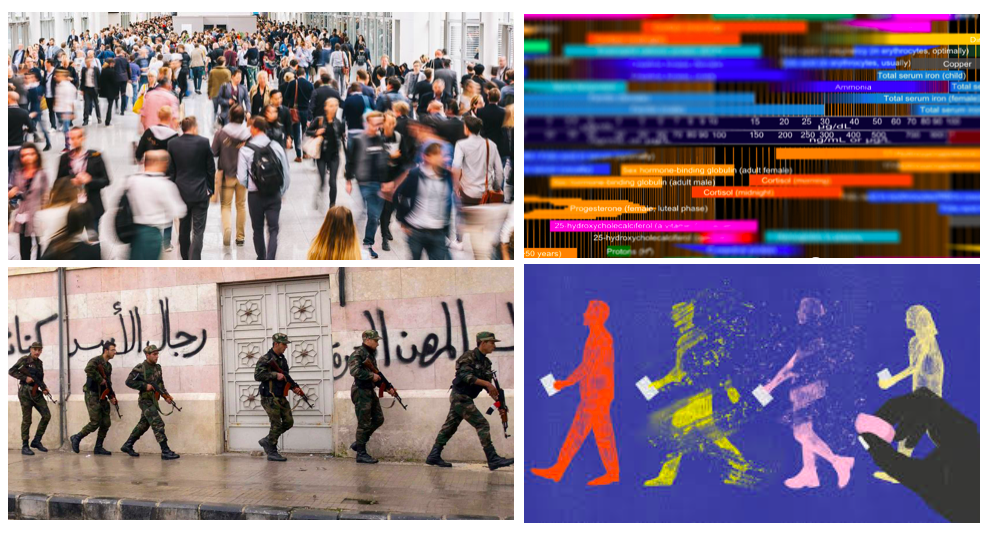
\includegraphics[scale=0.3]{figures/complex-data}

%\caption{default}
%\label{default}
\end{center}
\end{figure}


}

\frame{
\begin{figure}[htbp]
\begin{center}
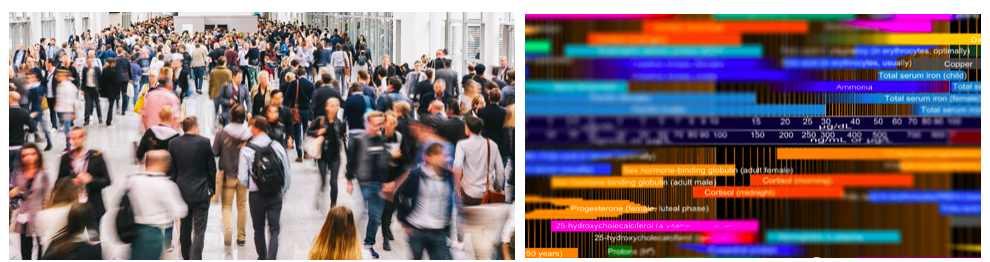
\includegraphics[scale=0.3]{figures/complex-data-top}
%\caption{default}
%\label{default}
\end{center}
\end{figure}

What do these datasets have in common?
\vspace*{1em}
\begin{itemize}
\item There is duplication in the data. 
\item The amount of duplication is typically small. 
\item Before we can apply inferential or prediction methods, any duplicate records must be removed.
\end{itemize}

}

\frame{
\frametitle{Data Cleaning Pipeline}



\begin{figure}[htbp]
\begin{center}
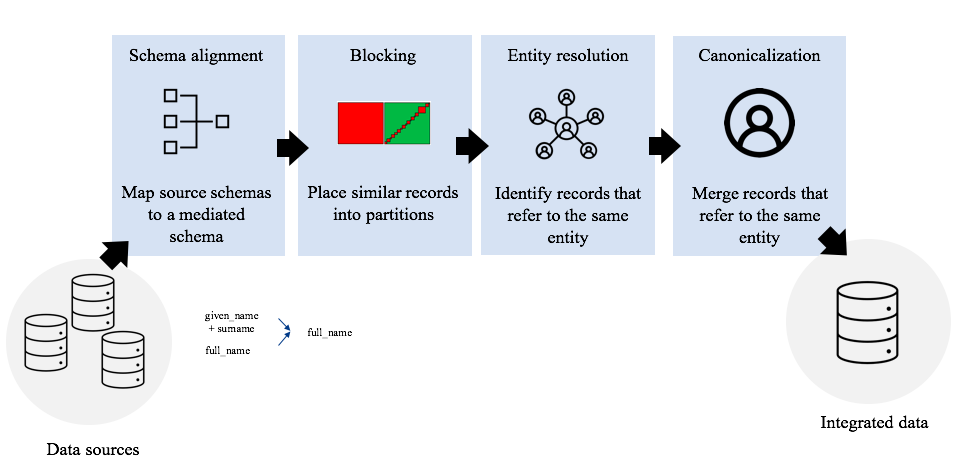
\includegraphics[scale=0.33]{finalFigures/pipeline}
%\caption{default}
%\label{default}
\end{center}
\end{figure}


}

\frame{

\Large
\center

Entity resolution (ER) is the process of merging together noisy (structured) databases to remove duplicate entities, often in the absence of a unique identifier.

}


\frame{

\Large
\center

Other names for entity resolution:  \\

\vspace*{1em}

record linkage, deduplication, duplicate detection, data matching, data integration, data cleansing.

}

%\frame{
%\frametitle{Data Cleaning Pipeline}
%
%
%
%\begin{figure}[htbp]
%\begin{center}
%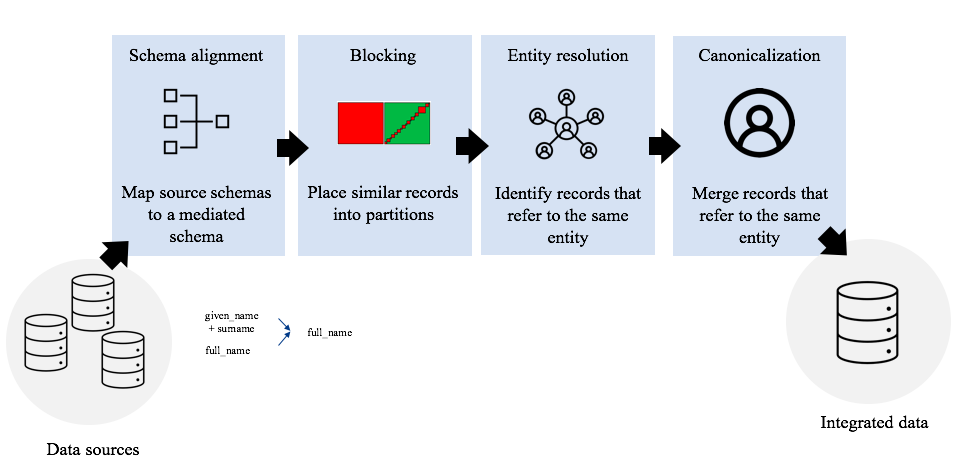
\includegraphics[scale=0.33]{finalFigures/pipeline}
%%\caption{default}
%%\label{default}
%\end{center}
%\end{figure}
%
%\center
%This talk focuses on blocking and entity resolution. 
%
%}

%\frame{
%\begin{figure}[htbp]
%\begin{center}
%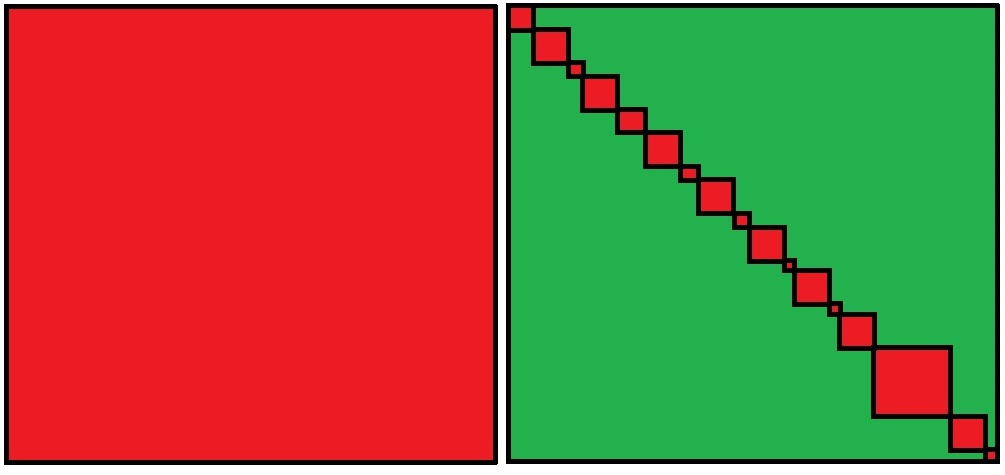
\includegraphics[scale=0.3]{finalFigures/block}
%%\caption{default}
%%\label{default}
%\end{center}
%\end{figure}
%
%\begin{center}
%\Large
%\emph{Blocking is the task of placing similar records into partitions in order to reduce the computational burden of the entity resolution task.}
%\end{center}
%}



%\frame{
%\begin{figure}[htbp]
%\begin{center}
%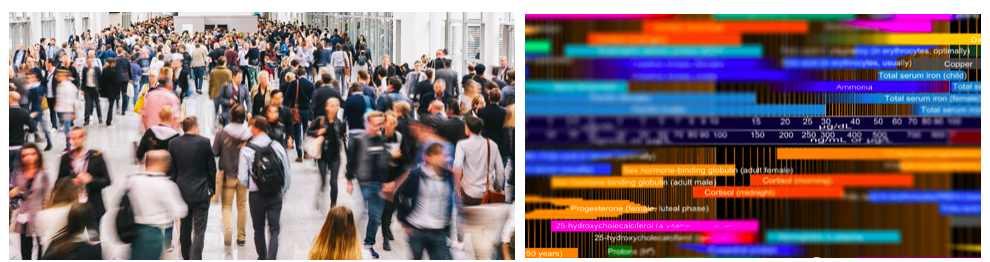
\includegraphics[scale=0.3]{figures/complex-data-top}
%%\caption{default}
%%\label{default}
%\end{center}
%\end{figure}
%
%\begin{center}
%\Large
%\emph{Entity resolution (record linkage or de-duplication) is the task of removing 
%duplicate entities from large noisy data sets, often in the absence of a unique identifier.}
%% (in the absence of a unique identifier). 
%\end{center}
%}

%\frame{
%\frametitle{Recent Work on Blocking}
%
%\begin{enumerate}
%\item Steorts+ (2014) proposed locality sensitive hashing (LSH) methods for blocking and provided comparisons to existing methods in the statistical machine learning literature. 
%\item Sadosky+ (2015) showed that most blocking methods are ill suited for human rights data. 
%\item Shrivastava and Steorts (2018) demonstrated the success of LSH on a case study provided by the Human Rights Data Analysis Group (HRDAG) to the Syrian conflict. 
%\item Edmorado and Steorts (2020) proposed the first approach of the Fellegi and Sunter method for probabilistic blocking that can feed into any entity resolution task. \end{enumerate}
%
%}







\frame{

\begin{center}
\Large
Foundations and Terminology
\end{center}

}

\frame{
\frametitle{A graph with no edges}
\begin{figure}[htbp]
\begin{center}
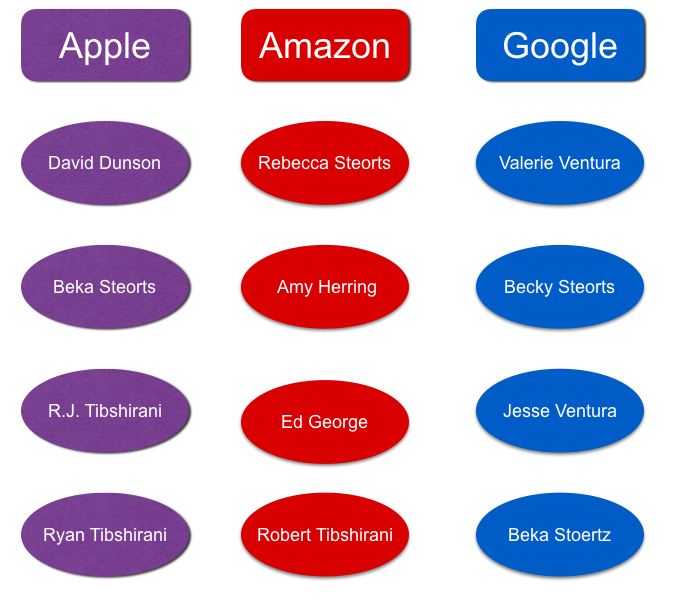
\includegraphics[scale=0.35]{pictures-new/graph-no-edges}
%\caption{default}
%\label{default}
\end{center}
\end{figure}



}

\frame{
\frametitle{The entity resolution graph}
\begin{figure}[htbp]
\begin{center}
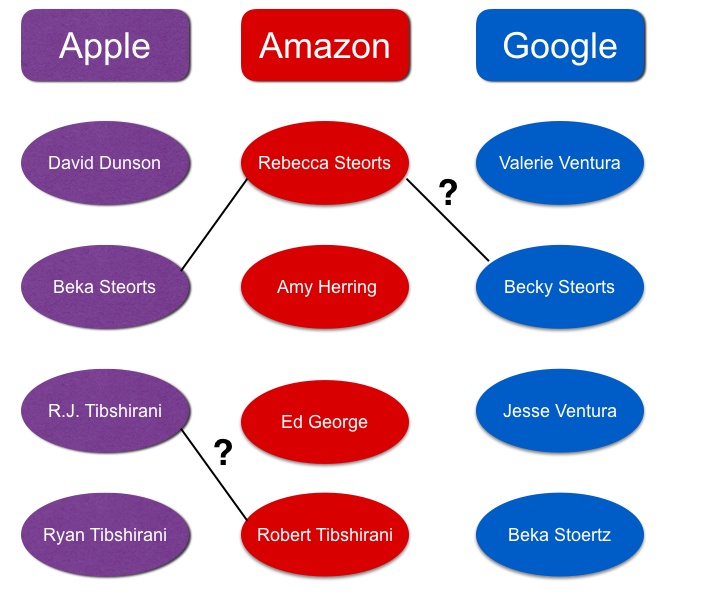
\includegraphics[scale=0.35]{pictures-new/graph}
%\caption{default}
%\label{default}
\end{center}
\end{figure}



}

\frame{
\frametitle{Entities are Real People (Objects, Businesses, Etc.)}
\begin{figure}[htbp]
\begin{center}
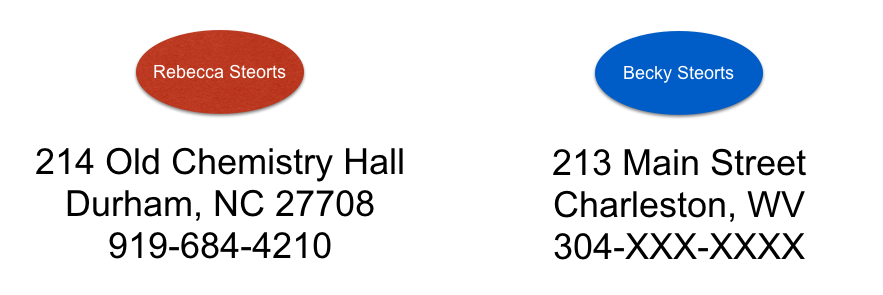
\includegraphics[scale=0.35]{pictures-new/node-two}
%\caption{default}
%\label{default}
\end{center}
\end{figure}



}

%\frame{
%\frametitle{Goal of Entity Resolution}
%
%\begin{figure}[htbp]
%\begin{center}
%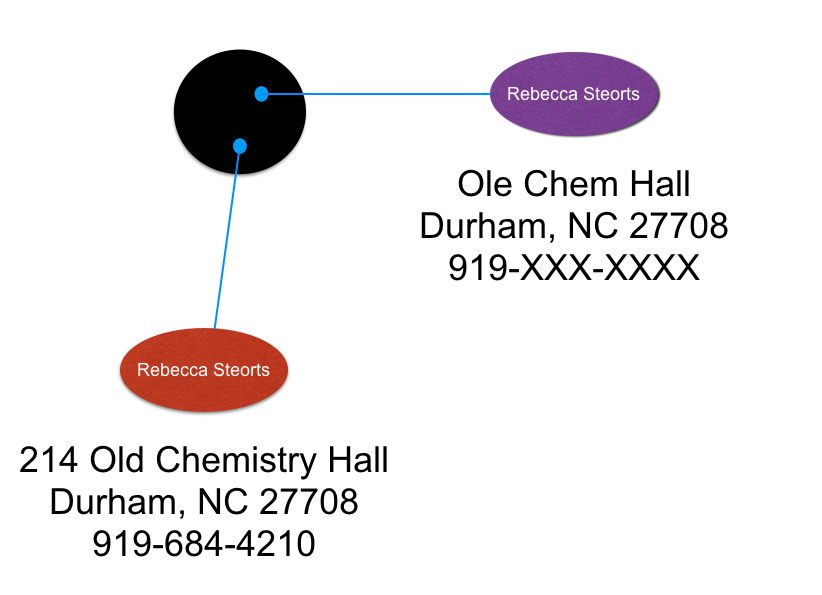
\includegraphics[width=0.6\textwidth]{pictures-new/output-er}
%%\caption{default}
%%\label{default}
%\end{center}
%\end{figure}
%
%%To find the most representative records after ER, one must perform canonicalization (data fusion or merging). 
%
%}

\frame{
\frametitle{Goal of Entity Resolution}

\begin{figure}[htbp]
\begin{center}
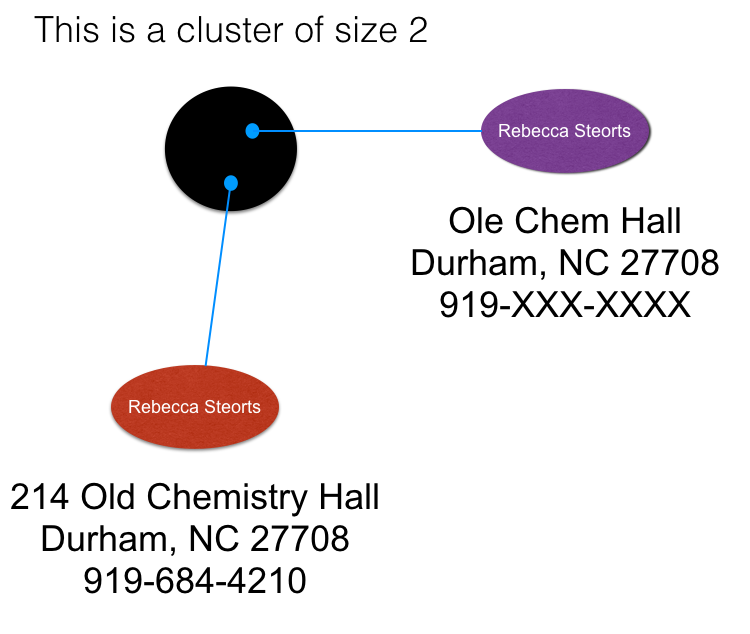
\includegraphics[width=0.6\textwidth]{pictures-new/microcluster}
%\caption{default}
%\label{default}
\end{center}
\end{figure}

%To find the most representative records after ER, one must perform canonicalization (data fusion or merging). 

}

\frame{
\frametitle{Goal of Entity Resolution}

\begin{figure}[htbp]
\begin{center}
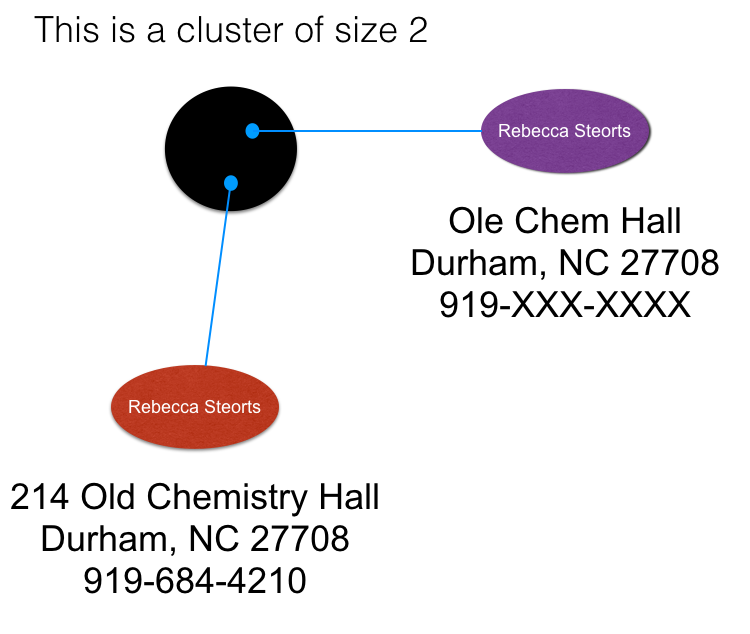
\includegraphics[width=0.6\textwidth]{pictures-new/microcluster}
%\caption{default}
%\label{default}
\end{center}
\end{figure}

To find the most representative records after ER, one must perform canonicalization (data fusion or merging). 

}

\frame{

\Large
\center

In this talk, I will focus on the entity resolution task of the data cleaning pipeline. 

\begin{figure}[htbp]
\begin{center}
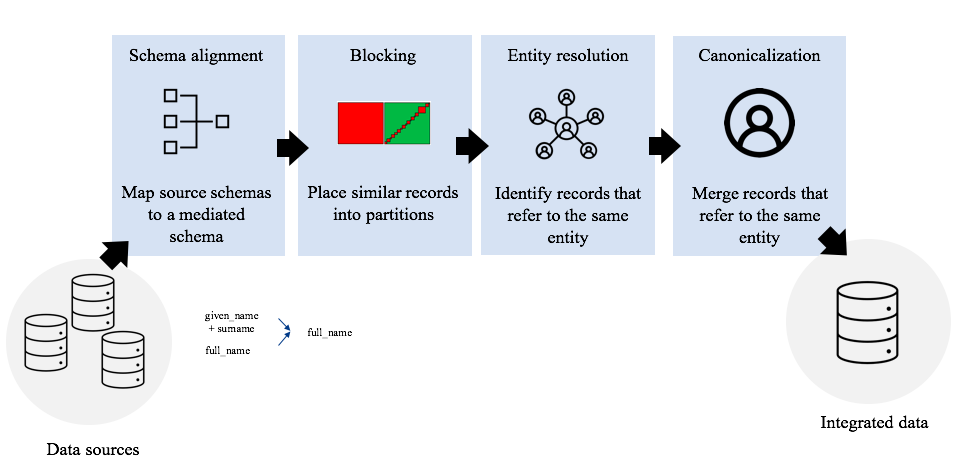
\includegraphics[width=0.9\textwidth]{finalFigures/pipeline}
%\caption{default}
%\label{default}
\end{center}
\end{figure}

%\vspace*{7em}

\normalsize

[Christen (2012), Christophides+ (2021), Papadakis+ (2021), Binette and Steorts (2022)]




}





\frame{
\center
\Large

Challenges

}

\frame{
\frametitle{Challenges of Entity Resolution}

\begin{figure}[htbp]
\begin{center}
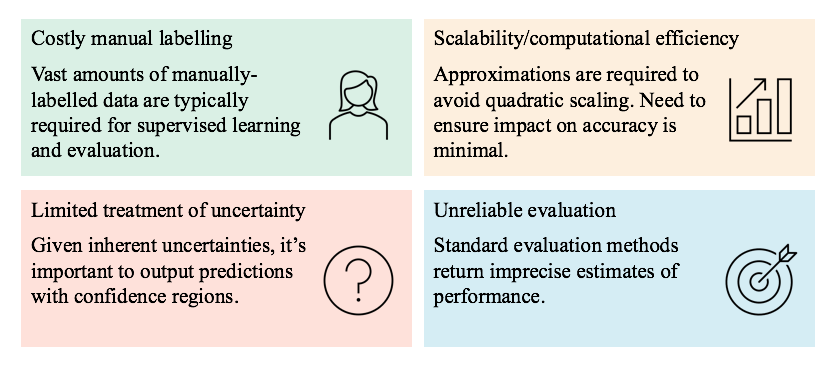
\includegraphics[scale=0.35]{finalFigures/pain-points}
%\caption{default}
%\label{default}
\end{center}
\end{figure}

}

\frame{
\frametitle{Evaluation Metrics}
\Large 

How do we assess the effectiveness of entity resolution methods, where some ground truth is known? 


}

\frame{
\frametitle{True Positive (True Matches)}


True Positive (TP): These are records that are classified as matches and are true matches. 

\vspace*{1em} These are pairs of records that refer to the same person (entity). 

}

\frame{
\frametitle{True Negatives (True Non-Matches)}

True Negative (TN): These record pairs are classified as non-matches, they are true non-matches.

\vspace*{1em} 

The two records refer to two different entities. 

}

\frame{
\frametitle{False Positive (False Matches)}


False Positive (FP): These are record pairs that have been classified as matches, but they are not true matches. 

%The model incorrectly predicted a positive match (the actual outcome was positive).

\vspace*{1em} 

The model made a wrong decision with the record pairs and falsely declared them to be matches. 

}



\frame{
\frametitle{False Negatives (False Non-Matches)}

These are record pairs that have been classified as non-matches, but they are actually true matches. 

\vspace*{1em} 


The two record pairs refer to the same entity, but the method made a mistake.



}

\frame{
\frametitle{Confusion Matrix}

\begin{itemize}
\item Match (M)
\item Non-Match (NM)
\item N = total records
\end{itemize}

 \begin{table}[htbp]
%\caption{Confusion Matrix}
\label{tab:confusion-matrix}
\centering
\renewcommand\arraystretch{1.2}
\begin{tabular}{|c|c|c|c|}\hline
\multirow{2}{*}{N}
    & \multicolumn{3}{c|}{Predicted}    \\
    \cline{2-4}
    &   & M & NM                     \\
  \hline
\multirow{2}{*}{Actual}
    &   M  &  \textcolor{purple}{TP}  (true matches)   &         \\
  \cline{2-4}
    &   NM &     &      \textcolor{purple}{TN} (true non-matches) \\
    \hline
\end{tabular}
    \end{table}
    
\begin{itemize}
\item True Positive (TP): The model correctly predicted a positive match (the actual outcome was positive).
\item True Negative (TN): The model correctly predicted a negative outcome (the actual outcome was negative).
\end{itemize} 

}

\frame{
\frametitle{Confusion Matrix}

\begin{itemize}
\item Match (M)
\item Non-Match (NM)
\item N = total records
\end{itemize}

 \begin{table}[htbp]
%\caption{Confusion Matrix}
\label{tab:confusion-matrix}
\centering
\renewcommand\arraystretch{1.2}
\begin{tabular}{|c|c|c|c|}\hline
\multirow{2}{*}{N}
    & \multicolumn{3}{c|}{Predicted}    \\
    \cline{2-4}
    &   & M & NM                     \\
  \hline
\multirow{2}{*}{Actual}
    &   M  &    &      \textcolor{purple}{FN}   \\
  \cline{2-4}
    &   NM &  \textcolor{purple}{FP}   &      \\
    \hline
\end{tabular}
    \end{table}
    
\begin{itemize}
\item False Positive (FP): The model incorrectly predicted that the record pairs are a true match. 
\item False Negative (FN): The model incorrectly predicted that the record pairs are a non-match. 
\end{itemize} 

}

\frame{
\frametitle{Confusion Matrix}

\begin{itemize}
\item Match (M)
\item Non-Match (NM)
\item N = total records
\end{itemize}

 \begin{table}[htbp]
%\caption{Confusion Matrix}
\label{tab:confusion-matrix}
\centering
\renewcommand\arraystretch{1.2}
\begin{tabular}{|c|c|c|c|}\hline
\multirow{2}{*}{N}
    & \multicolumn{3}{c|}{Predicted}    \\
    \cline{2-4}
    &   & M & NM                     \\
  \hline
\multirow{2}{*}{Actual}
    &   M  & \textcolor{purple}{TP}  (true matches)  &      \textcolor{purple}{FN}   \\
  \cline{2-4}
    &   NM &  \textcolor{purple}{FP}   &     \textcolor{purple}{TN} (true non-matches)  \\
    \hline
\end{tabular}
    \end{table}
    
%\begin{itemize}
%\item False Positive (FN): The model incorrectly predicted that the record pairs are a true match. 
%\item False Negative (FP): The model incorrectly predicted that the record pairs are a non-match. 
%\end{itemize} 

}


%\frame{
%\frametitle{Confusion Matrix}
%
%\begin{itemize}
%\item No = Non-Match
%\item Yes = Match
%\end{itemize}
%
% \begin{table}[htbp]
%\caption{Confusion Matrix}
%\label{tab:confusion-matrix}
%\centering
%\renewcommand\arraystretch{1.2}
%\begin{tabular}{|c|c|c|c|}\hline
%\multirow{2}{*}{N= Total Records}
%    & \multicolumn{3}{c|}{Actual}    \\
%    \cline{2-4}
%    &   & No & Yes                      \\
%  \hline
%\multirow{2}{*}{Predicted}
%    &   No  &   true neg. (TN)   & false neg. (FN)       \\
%  \cline{2-4}
%    &   Yes &  false pos.  (FP)  &  true pos. (TP)       \\
%    \hline
%\end{tabular}
%    \end{table}
%    
%In the TP, FP, TN, FN terminology:
%\begin{itemize}
%\item True Positive (TP): The model correctly predicted a positive match (the actual outcome was positive).
%\item True Negative (TN): The model correctly predicted a negative outcome (the actual outcome was negative).
%%\item False Positive (TP): The model incorrectly predicted a positive outcome (the actual outcome was negative).
%%\item ``True”/“False" = \textcolor{purple}{prediction} is correct/incorrect
%%\item   ``Positive”/“Negative" = predicted class is positive/negative
%\end{itemize} 
%
%}

%\frame{
%\frametitle{Confusion Matrix}
%
%\begin{itemize}
%\item No = Non-Match
%\item Yes = Match
%\end{itemize}
%
% \begin{table}[htbp]
%\caption{Confusion Matrix}
%\label{tab:confusion-matrix}
%\centering
%\renewcommand\arraystretch{1.2}
%\begin{tabular}{|c|c|c|c|}\hline
%\multirow{2}{*}{N= Total Records}
%    & \multicolumn{3}{c|}{Actual}    \\
%    \cline{2-4}
%    &   & No & Yes                      \\
%  \hline
%\multirow{2}{*}{Predicted}
%    &   No  &   true neg. (TN)   & false neg. (FN)       \\
%  \cline{2-4}
%    &   Yes &  false pos.  (FP)  &  true pos. (TP)       \\
%    \hline
%\end{tabular}
%    \end{table}
%    
%In the TP, FP, TN, FN terminology:
%\begin{itemize}
%\item False Positive (TP): The model incorrectly predicted a positive outcome (the actual outcome was negative).
%\item False Negative (FN): The model incorrectly predicted a negative outcome (the actual outcome was positive). 
%\end{itemize} 
%
%}


%\frame{
%\frametitle{Confusion Matrix}
%
%
% \begin{table}[htbp]
%\caption{Confusion Matrix}
%\label{tab:confusion-matrix}
%\centering
%\renewcommand\arraystretch{1.2}
%\begin{tabular}{|c|c|c|c|}\hline
%\multirow{2}{*}{}
%    & \multicolumn{3}{c|}{Predicted Linkage}    \\
%    \cline{2-4}
%    &   & Match & Non-Match                     \\
%  \hline
%\multirow{2}{*}{Actual Linkage}
%    &   Match  &  true pos. (TP)   &   false pos.  (FP)    \\
%  \cline{2-4}
%    &   Non-Match &  false neg. (FN)    &  true neg. (TN)       \\
%    \hline
%\end{tabular}
%    \end{table}
%    
%\vspace*{3em}    
%    
%In the TP, FP, TN, FN terminology:
%\begin{itemize}
%\item ``True”/“False" = \textcolor{purple}{actual linkage} is correct/incorrect
%\item   ``Positive”/“Negative" = predicted class is positive/negative
%\end{itemize}  
%
%}


\frame{
\frametitle{Evaluation Metrics}

Accuracy (acc) = $\dfrac{TP + TN}{TP + FP + TN + FN}$

\vspace*{2em}

\begin{itemize}
\item Commonly used in machine learning problems. 
\item Useful in situations where the data is balanced, i.e. matches and non-matches are roughly the same.
\item The number of TN dominates, and leads to a class imbalance issue (and results that are misleading).
\end{itemize}

\vspace*{2em}

For an example, see page 167 of Christen (2012).

}

\frame{
\frametitle{Evaluation Metrics}

\begin{itemize}
\item False positive rate (FPR) = $\dfrac{FP}{FP + TN}$
\begin{itemize}
\item Fraction of actual negatives that were predicted to be positive.
\end{itemize}
\item True Positive Rate (TPR) =  $\dfrac{TP}{TP + FN}$
\begin{itemize}
\item  Fraction of actual positives that were predicted to be positive.
\item Sensitivity = TPR. 
\end{itemize}
\item True negative rate (TNR) = specificity = $\dfrac{TN}{TN + FP}$
\end{itemize}
\vspace*{2em}
Which metrics suffer from a class imbalance issue and which ones do not?

%\vspace*{2em}

%\begin{itemize} 
%\item Useful in situations where the data is balanced, i.e. matches and non-matches are roughly the same.
%\item The number of TN dominates, and leads to a class imbalance issue (and results that are misleading).
%\end{itemize}

}

\frame{
\frametitle{Evaluation Metrics}

$$\text{Precision} = \dfrac{TP}{TP + FP}$$

\vspace*{2em}

Measures how precise a method is in classifying true matches.

$$\text{Recall} = \dfrac{TP}{TP + FN}$$

\vspace*{2em}

Measures how accurately the actual true matching pairs of records are correctly classified as matches. 


\vspace*{2em}
Observe these metrics do not include TN. They do not suffer from a class imbalance issue. 

}

\frame{
\frametitle{Evaluation Metrics}

$$\text{F-Measure} = \dfrac{2\times \text{Precision} \times \text{Recall}}{ \text{Precision} + \text{Recall}}$$

\begin{itemize}
\item Harmonic mean of the precision and recall.
\item Attempts to summarize all aspects of the effectiveness of an entity resolution method.
\end{itemize}

}

\frame{
\frametitle{Summary}

\begin{itemize}
\item What is entity resolution (and other names for it)?
\item What are challenges of entity resolution? 
\item Know the components of a confusion matrix. 
\item What are the evaluation metrics used for entity resolution (and ones that we do not consider)? Be sure to know why! 
\end{itemize}

}






\end{document}